\documentclass[10pt]{article}
\usepackage[polish]{babel}
\usepackage[utf8]{inputenc}
\usepackage[T1]{fontenc}
\usepackage{amsmath}
\usepackage{amsfonts}
\usepackage{amssymb}
\usepackage[version=4]{mhchem}
\usepackage{stmaryrd}
\usepackage{graphicx}
\usepackage[export]{adjustbox}
\graphicspath{ {./images/} }

\title{Zadania - etap II }

\author{}
\date{}


\begin{document}
\maketitle
(klasy 7 i 8 szkoły podstawowej i klasa III gimnazjum)\\
Zadanie 1. Gdyby Aleksander Wielki umarł o 5 lat wcześniej, to panowałby przez \(\frac{1}{4}\) swego życia. Gdyby żył o 9 lat dłużej, to panowałby przez połowę swego życia. Ile lat żył a ile lat panował Aleksander Wielki?

Zadanie 2. Wykaż, że jeśli \(a>1 \mathrm{i} b>1\), to: \(\frac{a}{b+1}+\frac{b}{a+1}>1\).\\
Zadanie 3. Dla liczby naturalnej \(n\) przez \(p(n)\) oznaczmy iloczyn cyfr liczby \(n\). Na przykład: \(p(7)=7, p(29)=2 \cdot 9=18, p(345)=3 \cdot 4 \cdot 5=60\). Oblicz: \(p(1)+p(2)+p(3)+\ldots+p(100)\).

Zadanie 4. Wewnątrz trójkąta równobocznego ABC o boku długości \(a\) obrano dowolnie punkt P i zrzutowano go prostopadle na boki AB, BC i AC, otrzymując odpowiednio punkty \(\mathrm{K}, \mathrm{L}, \mathrm{M}\). Oblicz, ile wynosi suma długości: \(|\mathrm{KP}|+|\mathrm{LP}|+|\mathrm{MP}|\).\\
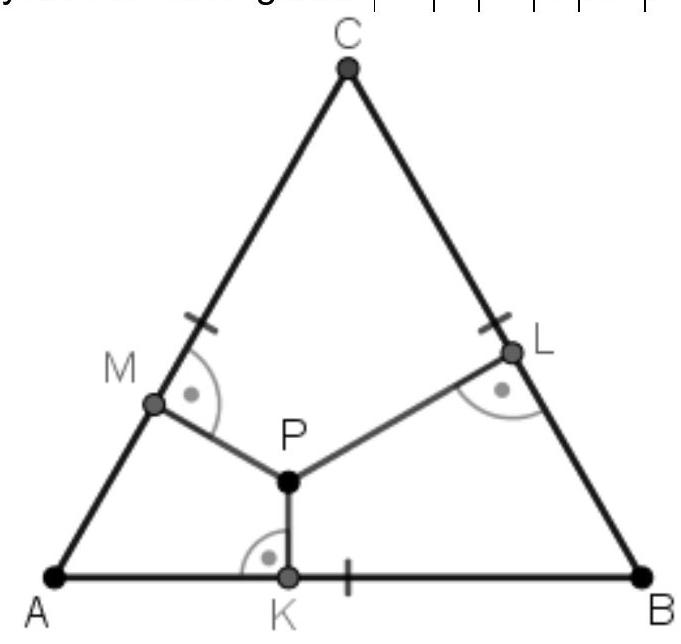
\includegraphics[max width=\textwidth, center]{2024_11_21_0d37590029f311fe3dcdg-1}

Zadanie 5. Rozwiąż układ równań:

\[
\left\{\begin{array}{l}
x+y+z=14 \\
x+y+t=10 \\
x+z+t=12 \\
y+z+t=15
\end{array}\right.
\]


\end{document}